%
To tackle the problem of flexible privacy in web applications, we present a
system design that moves closer to an Internet where users can leave services
and return at any time, where old data on servers is protected by default, and
where services provide users with control over their identifying data visible to
the service and other users.
%
We capture this goal with the new key abstraction of \emph{disguised data}.
Disguised data represents a state of data where \one{} some or all of the user's
original sensitive data is rendered inaccessible to the application; \two{} some
data may be replaced with placeholders to keep the application structure intact
(\eg placeholder parent comments to maintain comment thread structure); and
\three{} the data can be restored with the user's authorization.
%

To realize disguised data, we present a general system that helps developers
specify and apply two kinds of transformations: \emph{\xxing transformations},
which move the user's data into a disguised state; and \emph{revealing
transformations}, which restore the original data at a user’s request.
%
\Xxing transformations aim to protect the confidentiality of users' \xxed data
(\eg links to throwaway accounts or old HotCRP reviews) even if the application
is later compromised (\eg via a SQL injection or a compromised admin's account).
%

%
We demonstrate our approach in \sys, a system that realizes disguising and
revealing transformations for database-backed web applications via a set of
primitives that have well-defined semantics and compose cleanly.
%
Developers specify the transformations that their application should provide,
and \sys takes care of correctly applying, composing, and optionally reverting
them, while maintaining application functionality and referential integrity.
%

%
\subsection{Challenges}
%
We had to address three challenges to make this approach work.
%
First, \sys needs to present a simple, yet versatile interface for developers to
specify \xxing transformations.
%
\sys addresses this challenge with a restricted programming model centered
around three primitives: remove, modify, and decorrelate (which reassigns data
to placeholder users).
%
This model limits the potential for developer error, and lets \sys derive the
correct \xxing and revealing operations, while supporting a wide range of
transformations.
%

%
Second, to work with existing applications in practice, \sys's \xxing
transformations should require minimal application modifications.
%
To achieve this, \sys introduces \emph{pseudoprincipals}, anonymous placeholder
users that are inserted into the database on \xxing and exist solely to own data
decorrelated from real users (\eg because the application requires the data to
continue operating) and maintain referential integrity.
%
Pseudoprincipals can also act as built-in ``throwaway accounts,'' as they let
the user disown data after-the-fact, as well as potentially later reassociate
with it.
%
To correctly reason about ownership when data may be decorrelated multiple times
(\eg by global anonymization after throwaways have been created), \sys maintains
an encrypted speaks-for chain of pseudoprincipals that only the original user
can unlock and modify.
%

%
Third, \sys needs to have access to the original data for users to be able to
reveal their data and return to the application, but the whole point is to make
that data inaccessible to the service.
%
While \sys could ask users to store their own \xxed data, this would be
burdensome.
%
Instead, \sys stores the \xxed data on the server in encrypted form, and unlocks
and restores data to the service only when a user provides their credentials to
reveal.
%

\subsection{\sys Overview}

\begin{figure}[t!]
  \centering
    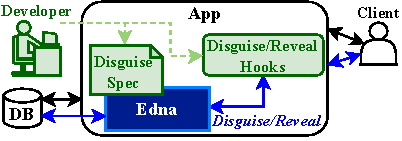
\includegraphics{figs/edna_overview}
    \caption{Developers write \xx specifications and add hooks to invoke \sys
        from the application (green); in normal operation, clients use these
        hooks in the application to \xx and reveal their data in the database
        (blue).
    }
  \label{f:edna-overview}
\end{figure}
%
\sys helps developers realize new options for users to control their data
via \emph{\xxing transformations}.
%
The developer integrates an application with \sys by writing \xx specifications
and adding hooks to \xx or reveal data using \sys's API
(Figure~\ref{f:edna-overview}).
%
This proceeds as follows:
%

%
(1) An application registers users with a public--private keypair
that either the application or the user's client generates; \sys stores the
public key in its database, while the user retains the private key for use in
future reveal operations.
%

%
(2) When the application wants to \xx some data, it invokes \sys with the
corresponding developer-provided \xx specification and any necessary
parameters (such as a user ID).
%
\Xx specifications can remove data, modify data (replacing some or all of its
contents with placeholder values), or decorrelate data, replacing
links to users with links to pseudoprincipals (fake users).
%
% Decorrelation preserves the structure of the application database, and avoids
% integrity issues like dangling foreign keys, while obscuring the data's
% relationship to natural principals (true users).
%
\sys takes the data it removed or replaced and the connections between
the user and any pseudoprincipals it created, encrypts that data with the user's
public key, and stores the resulting ciphertext---the \emph{\xxed
data}---such that it cannot be linked back to the user without the user's
private key.
%
%The application's database now no longer contains the \xxed data.
%

%
(3) When a user wishes to reveal their \xxed data, they pass credentials
to the application, which calls into \sys to reveal the data.
%
Credentials are application-specific: users may either provide their private
key or other credentials sufficient for \sys to re-derive the private key.
%
\sys reads the \xxed data and decrypts it, undoing the changes to the
application database that \xxing introduced.

%
\sys provides the developer with sensible default \xxing and revealing
semantics (\eg revealing makes sure not to overwrite changes made since
\xxing).

%%%%%%%%%%%%%%%%%%%%%%%%%%%%%%%%%%%%%%%%%%%%%%%%%%%%%%%%%%%%%%
\subsection{Example: Lobsters Topic Anonymization}
\label{s:design:lobsters}

\begin{figure}[t]
\centering
\begin{lstlisting}[style=rust,escapeinside={(*}{*)}]
// Decorrelate comments on stories w/tag {{TAG}}
"comments": [{
  "type": "Decorrelate",
  "predicate": "tags.tag = {{TAG}}",
  "from": "comments JOIN stories ON comments.story_id = stories.id
           JOIN taggings ON stories.id = taggings.story_id
           JOIN tags ON...",
  "group_by": "stories.id",
  "principal_fk": "comments.user_id" } ],
// Remove votes on stories w/tag {{TAG}}
"votes": [{
  "type": "Remove",
  "predicate": "tags.tag = {{TAG}}",
  "from": "votes JOIN stories...",
  "principal_fk": "votes.user_id",
}, ... ]
\end{lstlisting}
    \caption{Lobsters topic-based anonymization \xx specification (JSON
    pseudocode), which decorrelates comments and removes votes on stories with
    the specific topic tag.}
\label{f:spec}
\end{figure}



\begin{figure}[h]
  \centering
  \begin{subfigure}[h]{0.5\columnwidth}
  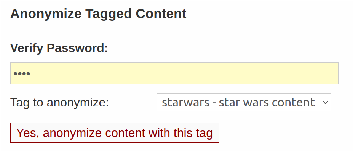
\includegraphics[width=\columnwidth]{figs/lobsters_catanon}
  \end{subfigure}
  \begin{subfigure}[h]{\columnwidth}
  \begin{lstlisting}[language=Ruby,escapeinside={(*}{*)}]
  def tag_anon
    # instantiate the disguise spec with the provided tag to anonymize
    disg_spec = edna.instantiate_spec("tag_anon.json",params[:tag])
    # apply the disguising transformation
    disg_id = edna.apply_disguise(@user.id,params[:passwd],disg_spec)
    # email the disguise ID to the user to allow revealing
    SendDisguiseEmail(@user, disg_id)
  end
  \end{lstlisting}
  \end{subfigure}
  \vspace*{-1em}
  \caption{The Lobsters developer adds a hook in the UI and code to perform
      topic-based anonymization.}
  \label{f:lobsters_hook}
  \end{figure}

Lobsters~\cite{lobsters} is a link-sharing and discussion platform with 15.4k
users.
%
Its database schema consists of stories, tags on stories, comments, votes,
private messages, user accounts, and other user-associated metadata.
%
Users create accounts, submit URLs as stories, and interact with other users
and their posted stories via comment threads and votes.
%

Consider \textbf{topic-based anonymization}, which allows users to
hide their interest in a topic (a ``tag'' in Lobsters) by decorrelating
their comments and removing their votes on stories with that tag.
%
For instance, a Lobsters user Bea who posts about their interests---Rust,
static analysis, and Star Wars---might want to hide associations with
Star Wars before sharing their profile with potential employers.
%
This is currently not possible in Lobsters.

%
The Lobsters developer can realize topic-based anonymization as a \xxing
transformation.
% that anonymizes Bea's contributions in the database, while allowing
% Bea to later edit and reclaim them if desired.
%
First, the developer writes a \xx specification that instructs \sys to
decorrelate comments and remove votes on ``Star Wars'' stories
(Figure~\ref{f:spec}), and provides it to \sys.
%
They also add frontend code and UI elements that allow authenticated users to
trigger the \xxing transformation (Figure~\ref{f:lobsters_hook}).
%
When Bea wants to anonymize their contributions on content tagged ``Star Wars'',
Lobsters invokes \sys with the provided specification .

%%%%%%%%%%%%%%%%%%%%%%%%%%%%%%%%%%%%%%%%%%%%%%%%%%%%%%%%%%%%%%%%%%%%%%
\subsection{Threat Model}
\label{s:threat}
%
%\sys assumes well-intentioned developers who follow standard security practices
%(\eg password protections)
%and write \xx specifications that capture the desired application semantics.
%
%\sys \xxs data according to these specifications, but because the database
%retains some data,
%to keep application semantics intact,
%\sys cannot protect against statistical correlation attacks.
%provide information-theoretic privacy guarantees.
%
\sys protects the confidentiality of \xxed data between the time when a user
disguises their data and the time when they reveal it.
%
%(where \xxed data is defined by the trusted developer-provided disguise specification).
%
During this period, \sys ensures that the application cannot learn the contents of
disguised data, nor learn what \xxed data corresponds to which user, even if the
application is compromised and an attacker dumps the database contents (\eg via
SQL injection).
%
\sys stores \xxed data encryptedly, so its confidentiality stems from ``crypto
shredding,'' a GDPR-compliant data deletion approach based on the fact that
ciphertexts are indistinguishable from garbage data if the key material is
unavailable~\cite{dnefs,townsend:cryptoshredding,aws:cryptoshredding,gtr:cryptoshredding}.
%

% STANDARD CLAIMS ABOUT CRYPTO ASSUMPTIONS
%
We make standard assumptions about the security of cryptographic primitives:
attackers cannot break encryption, and keys stored with clients are safe.
%
If a compromised application obtains a user's credentials, either because the
user provides them to the application for reveal, or via external means such as
phishing, \sys provides no guarantees about the user's current or future
disguised data.
%
\sys also expects the application to protect backups created prior to disguising;%
\footnote{If the application restores a backup, \sys continues operating
as if only the transformations up to the time of the snapshot had been applied.}
and external copies of the data
(\eg Internet Archive or screenshots) are out of scope.
%

%
While \sys hides the contents of \xxed data and relationships between \xxed data
and users, it does not hide the existence of
\xxed data. (An attacker can see if
a user has \xxed some data, but cannot see which \xxed data corresponds to this
user.)
%
An attacker can also see any data left in the database, such as pseudoprincipal
data or embedded text.
%
\sys puts out of scope attacks that leverage this leftover data
and metadata to infer which principal originally owned which objects.
%

\sys's choice of threat model and its limitations stem from
\sys's goal of practicality and usability by existing applications, and
from design components that support this goal.
%
For example, decorrelation with pseudoprincipals removes explicit user-content
links, but leaves placeholder information in the database to avoid application
code having to handle dangling references.
%
Similarly, leveraging server-side storage to hold \xxed data leaves
metadata available to attackers, but avoids burdening users with data storage
management.
